\vspace{10pt}

{\centering\subsection*{吴芷萱:大熊猫的自述}}

\addcontentsline{toc}{subsection}{吴芷萱:大熊猫的自述}

\renewcommand{\leftmark}{吴芷萱:大熊猫的自述}

\begin{figure}[htbp]

\centering

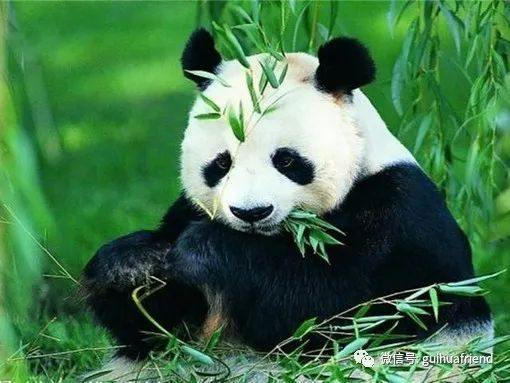
\includegraphics[width = .5\textwidth]{./ch/7.jpg}

\end{figure}



我是中国很特殊,很稀少的动物。我就是最可爱的、人见人爱的“大熊猫”。

我的全身都是毛茸茸的,圆嘟嘟的身体,还有一张圆圆的脸和一对圆圆的耳朵,还有一对八字形的黑眼圈,好似带着一副墨镜,非常招人喜欢。你觉得我长得可爱吗?

我最喜欢在草地上和同伴们一起嬉戏打闹。我们熊猫喜欢挠人,喜欢趴在树上睡觉,我们很喜欢用手捆住饲养员的脚,扒着不放,每次饲养员都是一拽一拽的,走出去的。不过我们也很容易生气,一生气就会狠狠的挠你的,我们喜爱吃竹子和竹笋等,有时会吃一些肉。

我们住在四川,陕西,甘肃等地,四川是我们熊猫的基地。欢迎你们来看我!

我们喜欢在草地和竹林上玩,我们熊猫数量稀少,野生的熊猫不足1600只,在中国有八万年的历史,所以有了“活化石”的称号。最终我们被中国称为了国家一级保护动物,被称为“国宝”。我感到非常自豪。

我们还常常担任着“和平大使”的角色,带着中国人民的友谊,远渡重洋到国外交朋友,深受全世界的喜爱!





\vspace{10pt}



作者: 三(1)班 吴芷萱



指导老师:谢婷



投稿:2021年6月8日



发表:2021年6月9日






                



\vspace{10pt}

\hline



